\begin{figure}[H]
  \begin{center}
    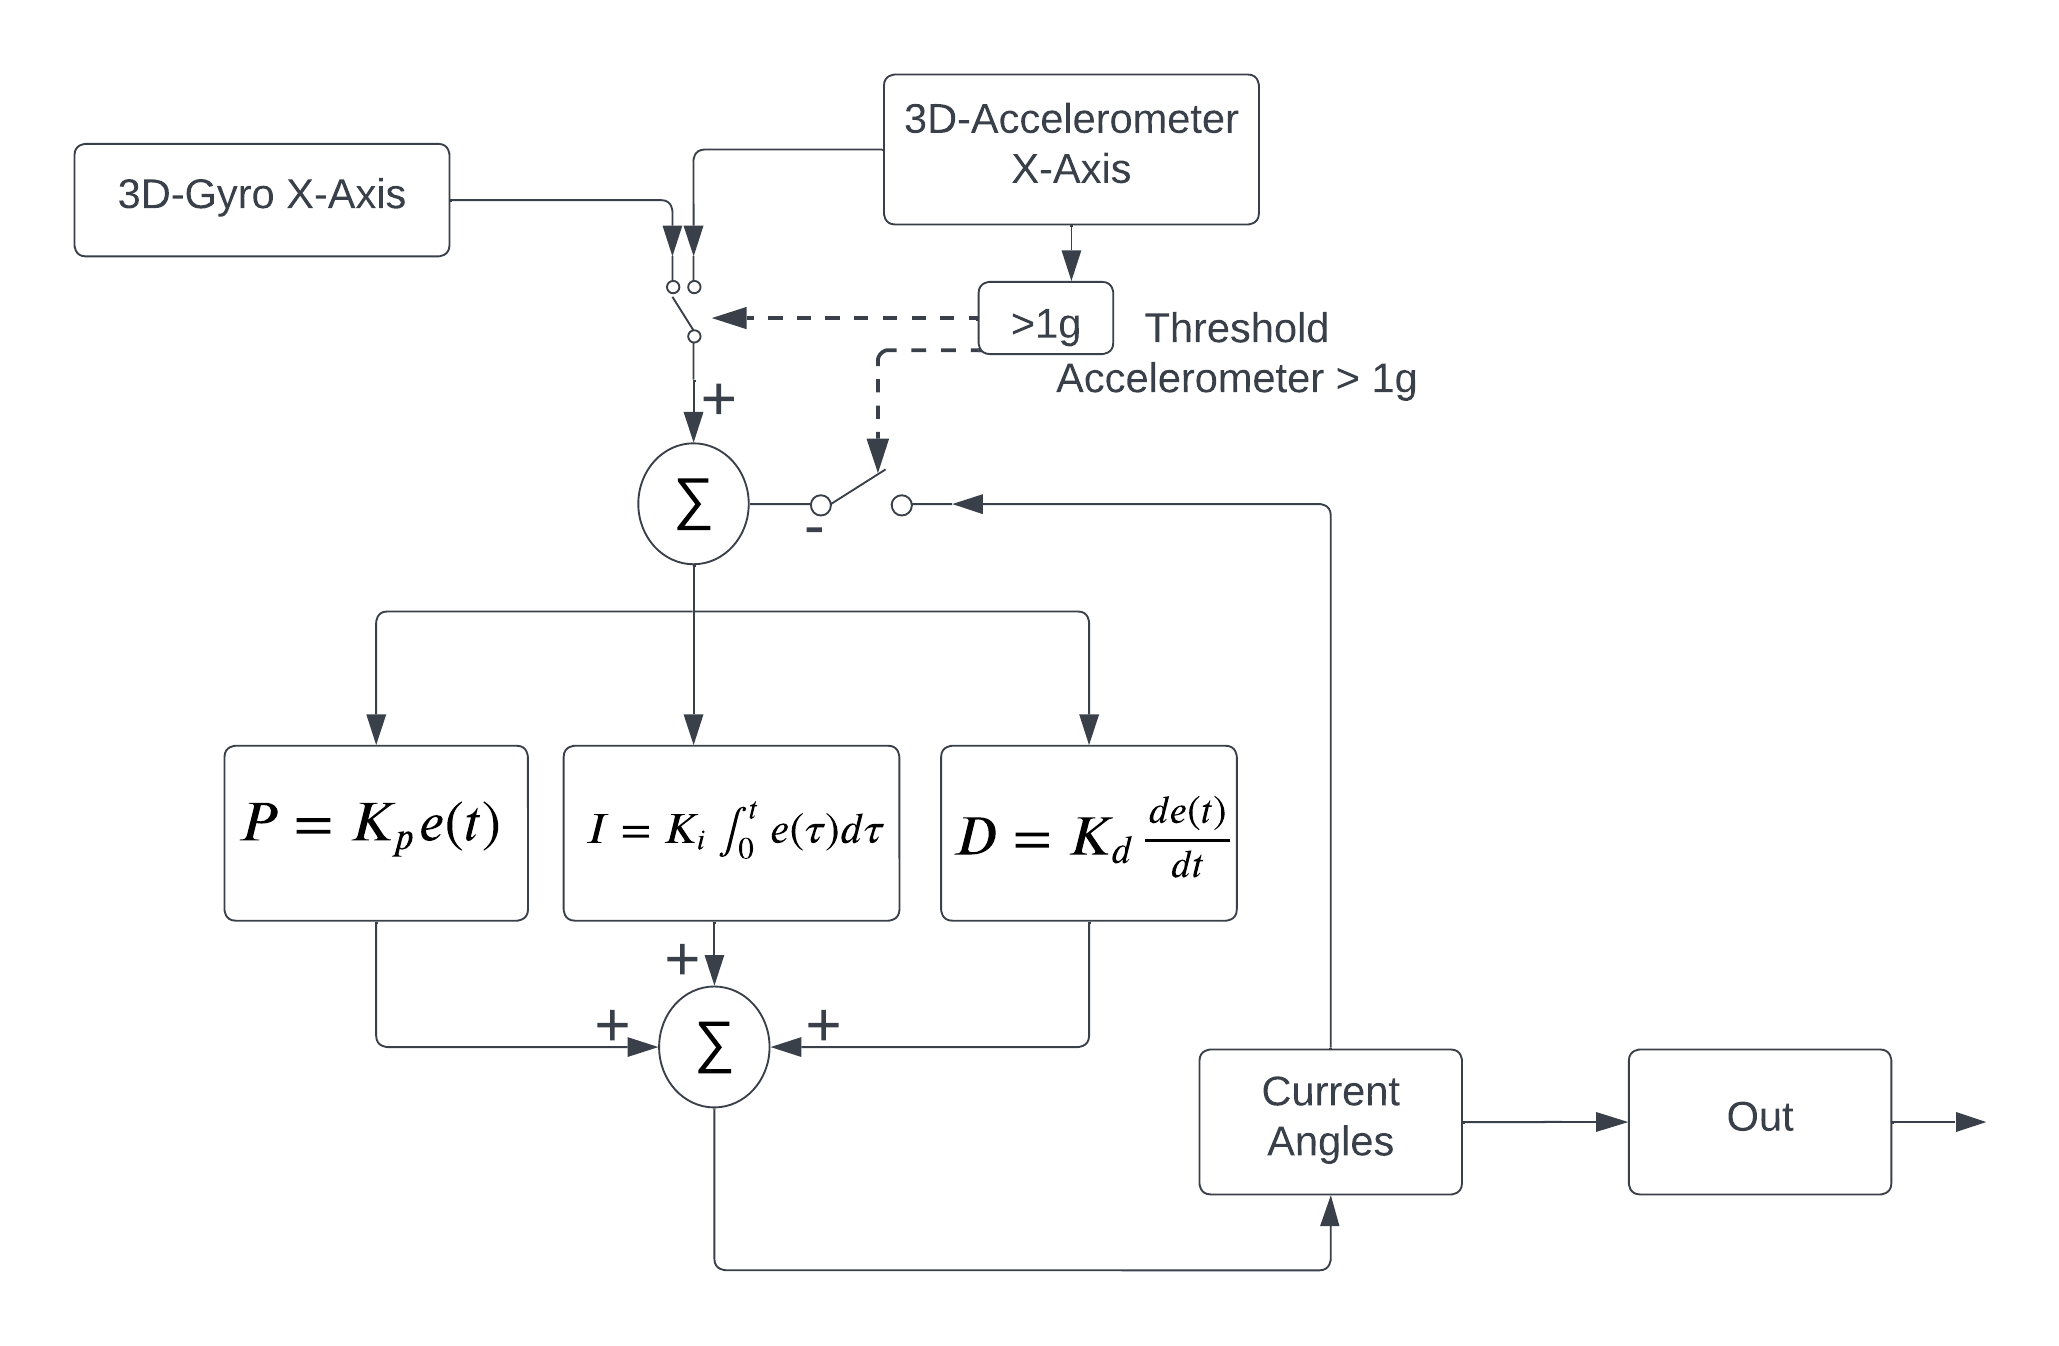
\includegraphics[width=1\linewidth]{content/images/PID_Loop.png}
    \caption{PID Loop}
  \end{center}
\end{figure}

\subsubsection{Algorythmus}
\begin{minipage}[l]{0.5\textwidth}
  \begin{math}
    Korrekturwert = K_p e(t) + K_i e_i \Delta{t} + \frac{K_d \Delta{e}}{\Delta{t}} \\
  \end{math} 
\end{minipage}
\begin{minipage}[r]{0.49\textwidth}
  \begin{table}[H]
    \centering
  \settowidth\tymin{Variablen}
  \setlength\extrarowheight{2pt}
  \begin{tabulary}{1.0\textwidth}{|L|L|}
    \hline
    \begin{math} K_p \end{math} & Proportional-Konstante\\
    \hline
    \begin{math} K_i \end{math} & Integral-Konstante\\
    \hline
    \begin{math} K_d \end{math} & Ableitung-Konstante\\
    \hline
    \begin{math} e(t) \end{math} & aktueller Fehler\\
    \hline
    \begin{math} \Delta{t} \end{math} & Zeit seit der letzten Korrektur\\
    \hline
    \begin{math} \Delta{e} \end{math} & Differenz des aktuellen und letzten Fehlers\\
    \hline
    \begin{math} e_i \end{math} & Fehlerintegral (\begin{math} \int_{0}^t e(t) \end{math})\\
    \hline
  \end{tabulary}
  \caption{Variablen Verzeichnis}
\end{table}
\end{minipage}

